\documentclass[tikz,11pt]{beamer}
\usepackage[utf8]{inputenc}
\usepackage[T1]{fontenc}
\usetheme{default}
\usepackage{lipsum}

% ----------------------------
% fabio - headers
% ----------------------------

\usepackage{tikz}
\usetikzlibrary{matrix,arrows.meta}

\begin{document}
\begin{frame}
	\frametitle{Objetivos do Trabalho}
\end{frame}

\begin{frame}
	\frametitle{Introdução e Motivação}
\end{frame}

\begin{frame}
	\frametitle{Apresentação do Bruno}
\end{frame}

\begin{frame}
	\frametitle{Apresentação do Bruno Canale}
\end{frame}

\begin{frame}
	\frametitle{Python - Keras Framework para Machine Learning}
\end{frame}

\begin{frame}
	\frametitle{Base de dados utilizada}
\end{frame}

\begin{frame}
	\frametitle{Implementação da Rede Convolucional}
\end{frame}

% -------------------------------------------------
% \begin{fabio}
% -------------------------------------------------

\begin{frame}
	\frametitle{Redes e Resultados}

    \begin{figure}
	\centering
	\begin{minipage}{.33\textwidth}
		\centering
		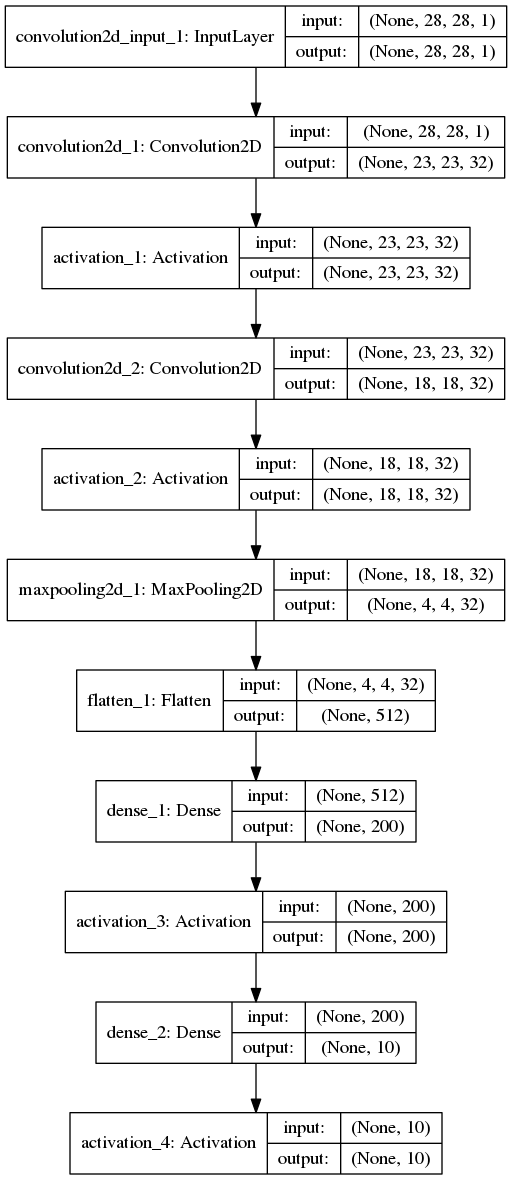
\includegraphics[width=.4\linewidth]{images/resultados/default/model}
	\end{minipage}%
	\begin{minipage}{.33\textwidth}
		\centering
		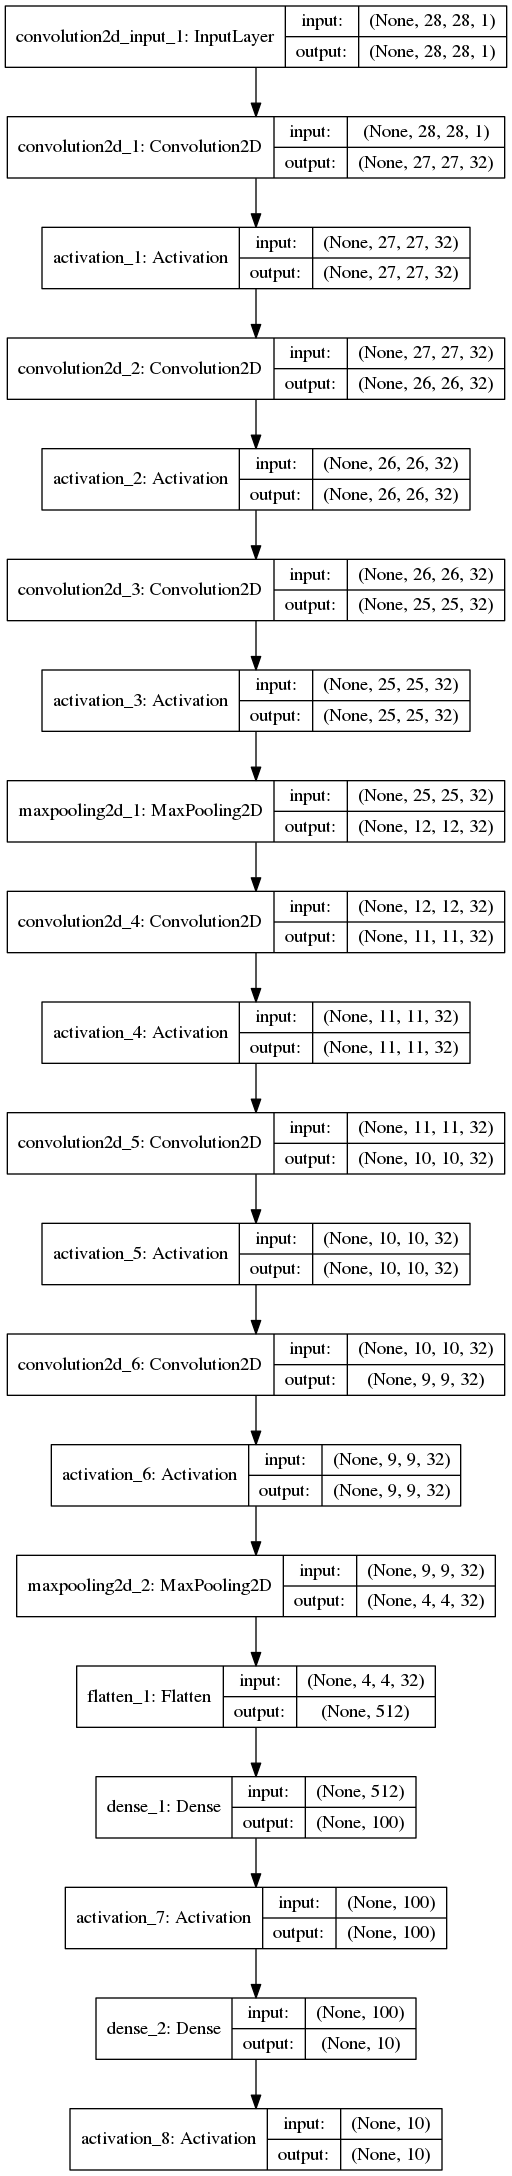
\includegraphics[width=.4\linewidth, height=.9\textheight]{images/resultados/network_1/model}
	\end{minipage}%
	\begin{minipage}{.34\textwidth}
	\centering
	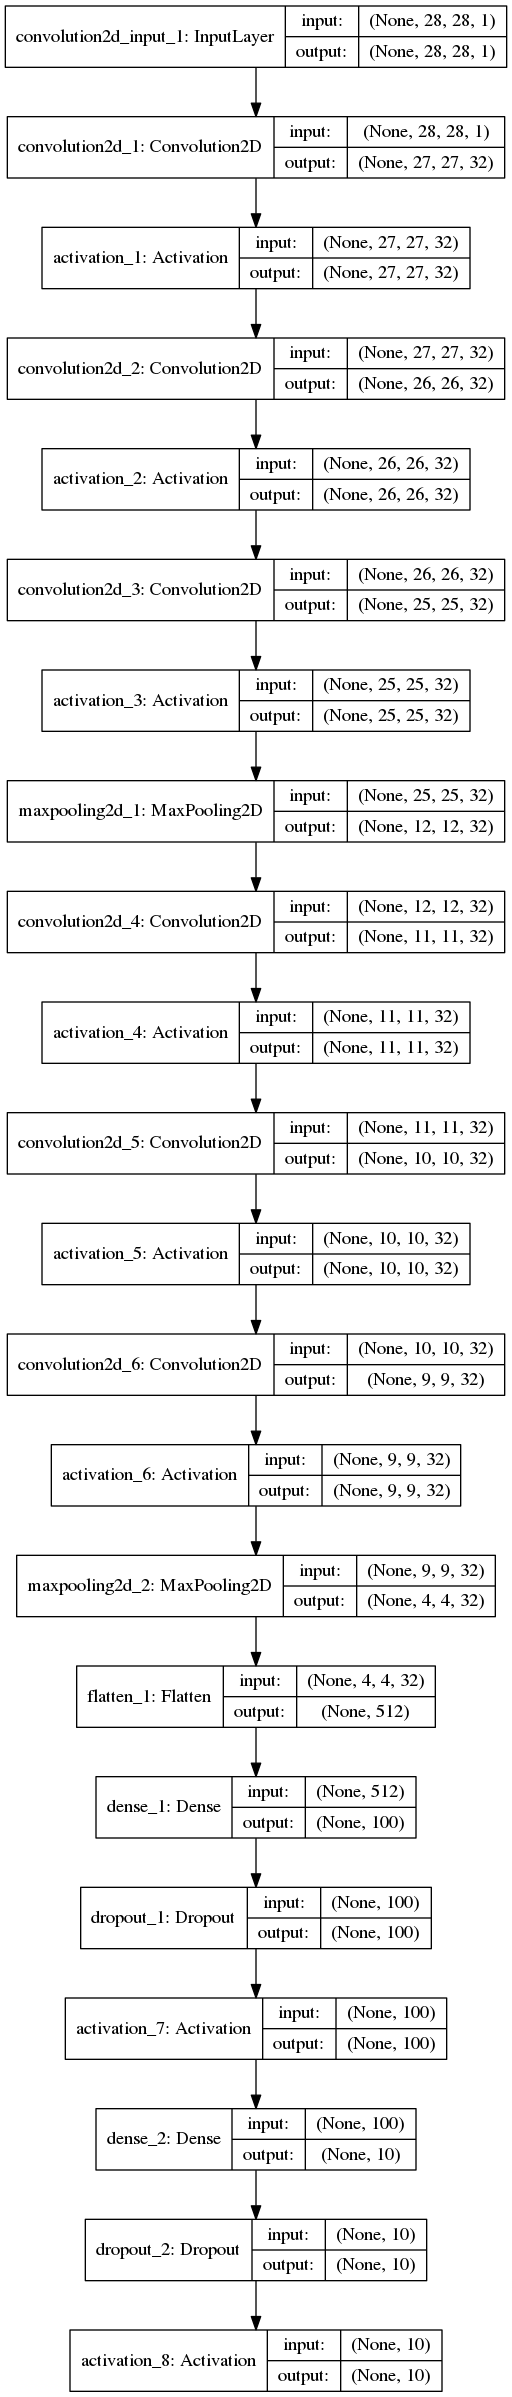
\includegraphics[width=.4\linewidth, height=.9\textheight]{images/resultados/network_2/model}
	\end{minipage}

\end{figure}

\end{frame}


\begin{frame}
	\frametitle{Camada de entrada}
	\centering
	MNIST DATASET
	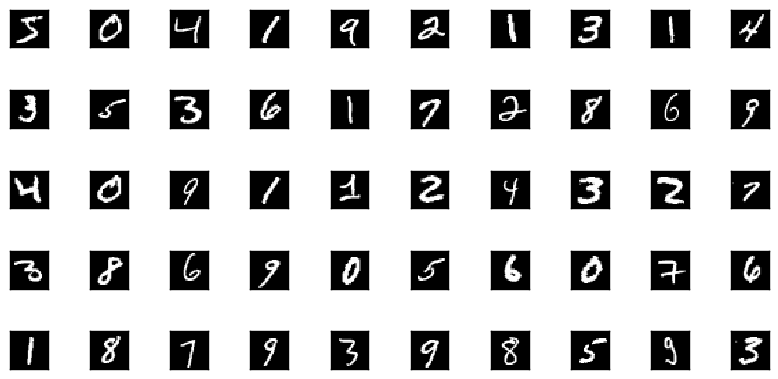
\includegraphics[width=.8\paperwidth]{images/fabio/inputs}
\end{frame}

\begin{frame}
	\frametitle{Primeira Rede - Arquitetura}
	\centering
	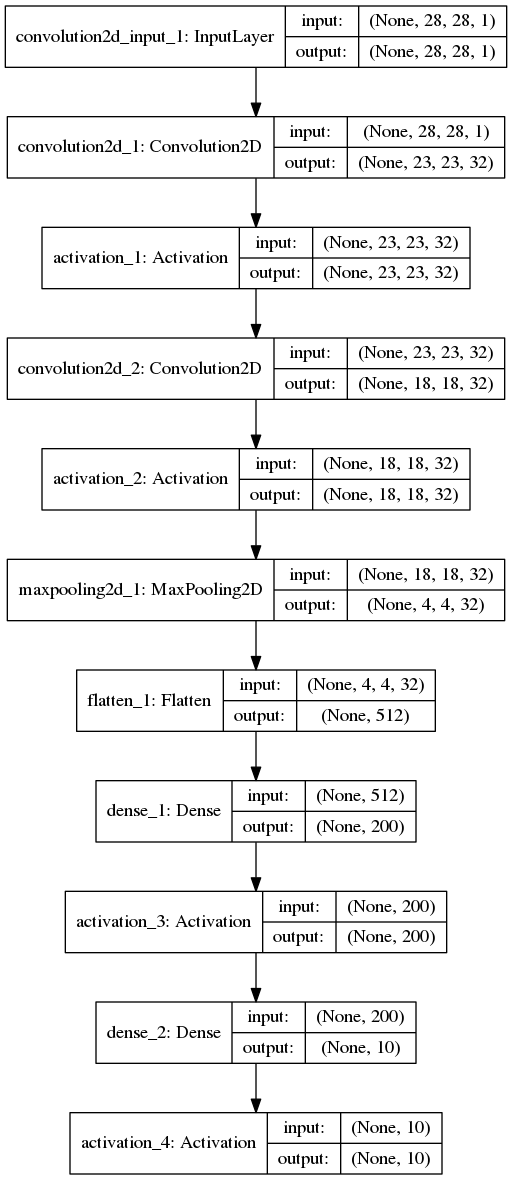
\includegraphics[height=.8\paperheight]{images/resultados/default/model}
\end{frame}

\begin{frame}
	\frametitle{Primeira Rede - Treinamento}
	\centering
	\begin{minipage}{.5\textwidth}
		\centering
		\par Treinamento:
		\begin{itemize}
			\item Épocas = 10
			\item Itens = 60000
		\end{itemize}		
	\end{minipage}%
	\begin{minipage}{.5\textwidth}
	\centering
	\par Teste
	\begin{itemize}
		\item Itens = 10000
	\end{itemize}		
\end{minipage}%

\end{frame}

\begin{frame}
	\frametitle{Convolução}
	\centering
	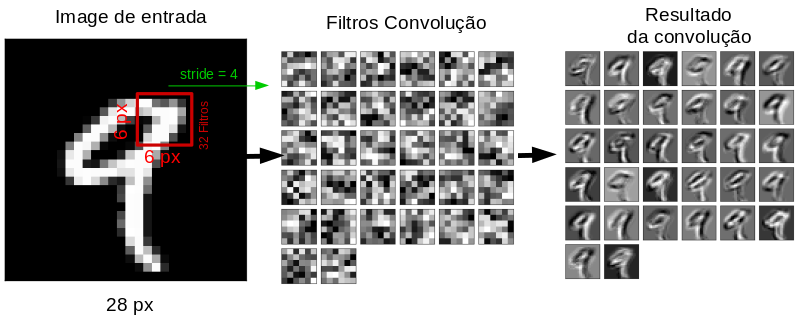
\includegraphics[width=.8\paperwidth]{images/fabio/conv_1}
\end{frame}

\begin{frame}
	\frametitle{Ativação}
	\centering
	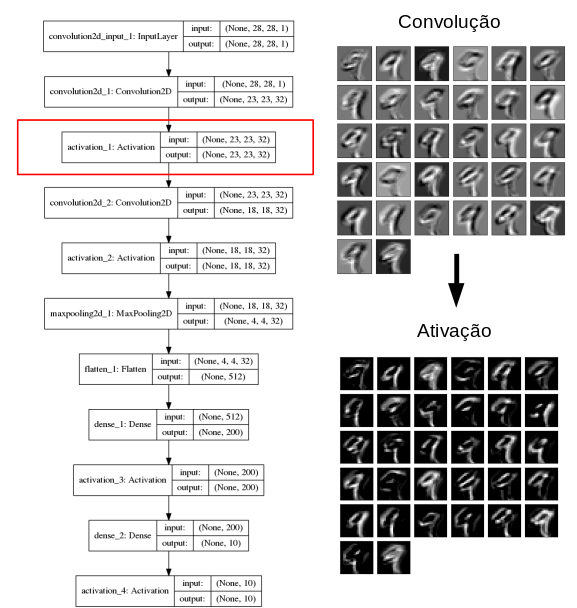
\includegraphics[height=.8\paperheight]{images/fabio/ativ_1}
\end{frame}


\begin{frame}
	\frametitle{Apresentacao do Fábio - Sugestão: Discussao sobre
		como essas observacoes ligam na MLP clássica e/ou problemas de
		Machine Learning}
\end{frame}
% -------------------------------------------------
% end{fabio}
% -------------------------------------------------
\end{document}